\documentclass[conference]{IEEEtran}
\usepackage{graphicx}
\usepackage{booktabs}
\usepackage{hyperref}
\usepackage{enumitem}
\usepackage{amsmath}
\begin{document}

\title{Improving Code Review via Clarification}
\author{
\IEEEauthorblockN{Saraswati Niroula}
\IEEEauthorblockA{saruniroula73@gmail.com}
}
\maketitle

\begin{abstract}
    Code review is essential for software quality, but AI reviewers struggle when pull request (PR) descriptions lack detail. Without context, they often produce vague feedback or hallucinate requirements. This study evaluates a simple intervention: introduce a clarification phase before review. Using ClarifyCoder to generate clarifying questions, supplemented with human answers, and then passing both the PR and Q\&A to Gemini, we compared baseline and clarified reviews across 12 PRs. Clarified reviews were consistently more specific, actionable, and higher in quality, while surfacing hidden assumptions and generating more useful suggestions. The results show that even a lightweight clarification step can significantly improve the effectiveness of AI-assisted code review.
\end{abstract}

\section{Introduction}
Code review is a cornerstone of modern software engineering practice. It improves code quality, enforces standards, and facilitates knowledge sharing among developers. However, the effectiveness of code review depends heavily on the clarity of pull request (PR) descriptions. When authors provide vague or underspecified information, reviewers are forced to guess the intended requirements, often leading to unhelpful or misleading comments. This problem is even more pronounced for AI-based reviewers, which lack the ability to actively request clarification from the author.

Large language models (LLMs) such as GitHub Copilot or Gemini have demonstrated the ability to generate natural-language review comments, but their effectiveness is tied directly to the information present in the PR description. Without sufficient context, these models frequently hallucinate constraints, remain overly generic, or fail to identify deeper issues that a human reviewer would naturally probe with questions. In other words, the inability to ask clarifying questions is a critical missing piece.

This project explores whether introducing a lightweight clarification step can address this gap. The core idea is to use a specialized model, ClarifyCoder, to generate targeted clarifying questions about ambiguous PRs. These questions are then answered manually, simulating the information exchange that typically occurs in human review conversations. The enriched context original PR plus Q\&A is then passed to Gemini, which acts as the reviewer.

By comparing baseline reviews (Gemini with only the PR description) against clarified reviews (Gemini with PR + clarifications), this study investigates whether reviews become more specific, actionable, and useful. The central hypothesis is that clarification improves review quality by grounding comments in explicit assumptions, reducing vagueness, and increasing actionable feedback.

\section{Background and Related Work}
Recent advances in large language models (LLMs) have highlighted both their potential and their limitations in software engineering tasks. While models such as GitHub Copilot and Gemini can generate and review code, they often struggle when faced with incomplete or ambiguous problem statements. In such cases, the models either hallucinate requirements or provide vague and generic reviews that are of limited use to developers.

ClarifyCoder \cite{wu2025clarifycoder} directly addresses this issue by fine-tuning models to ask clarifying questions before attempting problem solving. In their experiments, ClarifyCoder significantly improved program synthesis performance when task descriptions were underspecified. This demonstrates that a question-asking phase can effectively reduce ambiguity and improve downstream outcomes.

In the domain of code review, prior research has explored automation using both rule-based systems and LLMs. Rule-based approaches typically check for style violations, performance anti-patterns, or security flaws, but they lack flexibility in reasoning about high-level design intent. LLM-based approaches offer richer, more natural feedback but are hindered by the same lack of contextual grounding observed in program synthesis. 

By integrating ClarifyCoder with Gemini, this project adapts the idea of clarification from synthesis to review. Instead of asking models to guess missing information, a dedicated clarifier generates targeted questions. These questions are then answered by a human reviewer, supplying the missing context. The reviewing model, Gemini, can then leverage both the original PR description and the clarifications, leading to reviews that are more specific, actionable, and aligned with developer intent.

This work therefore extends ClarifyCoder’s contributions into a new domain, showing that clarification not only helps models write better code but also helps them review code more effectively.

\section{Problem Statement}
AI-based code reviewers show promise for assisting developers, but they face a fundamental limitation: the inability to request additional context. Unlike human reviewers, who naturally ask clarifying questions when PR descriptions are incomplete, current models either proceed with insufficient information or hallucinate requirements. This results in vague, generic, or even misleading feedback that fails to support developers effectively.

The challenge, therefore, is not only in generating review comments but in grounding them in the actual intent of the PR. Without explicit clarifications, reviews lack specificity, offer limited actionable guidance, and carry a high assumption rate. These shortcomings undermine the usefulness of automated reviews and highlight the need for an intermediate step that bridges the information gap.

This work frames the problem as follows: \emph{Can introducing a clarification phase, where an LLM generates targeted questions and receives answers improve the quality of AI-generated code reviews?} If effective, such an approach would shift reviews from vague commentary toward actionable, assumption-free feedback, aligning more closely with the standards of human review practice.

\section{Methodology}
The study was conducted in a controlled experimental workflow designed to evaluate the impact of clarification on AI code review. The process was implemented in several clearly defined steps.

\subsection{Workflow}
The overall pipeline consisted of the following stages:
\begin{enumerate}[leftmargin=*]
    \item \textbf{Dataset preparation:} Twelve representative pull requests (PRs) were constructed to cover a variety of common review scenarios, including logic changes, feature additions, and security-related fixes. Each PR was stored in JSONL format for reproducibility.
    \item \textbf{Clarification:} The ClarifyCoder model \cite{wu2025clarifycoder} was used in “ask” mode to generate clarifying questions for each PR description. This step simulated how a human reviewer probes missing requirements.
    \item \textbf{Answering:} The clarifying questions were answered manually, from the perspective of a senior reviewer. This ensured consistent, high-quality answers to supply to the reviewing model.
    \item \textbf{Review generation:} Two sets of reviews were produced using Gemini:
    \begin{itemize}[leftmargin=*]
        \item \textbf{Baseline:} Gemini reviewed the PR using only the original PR description.
        \item \textbf{Clarified:} Gemini reviewed the PR using both the PR description and the clarifying Q\&A.
    \end{itemize}
    \item \textbf{Comparison and scoring:} Reviews were stored side by side (\texttt{comparison.tsv}), and each PR was scored manually on five dimensions: specificity, actionability, assumption identification, comment quality, and suggestions. Scores were recorded in \texttt{eval\_scored.tsv} and aggregated into \texttt{eval\_summary.tsv}.
\end{enumerate}

\begin{figure}[t]
  \centering
  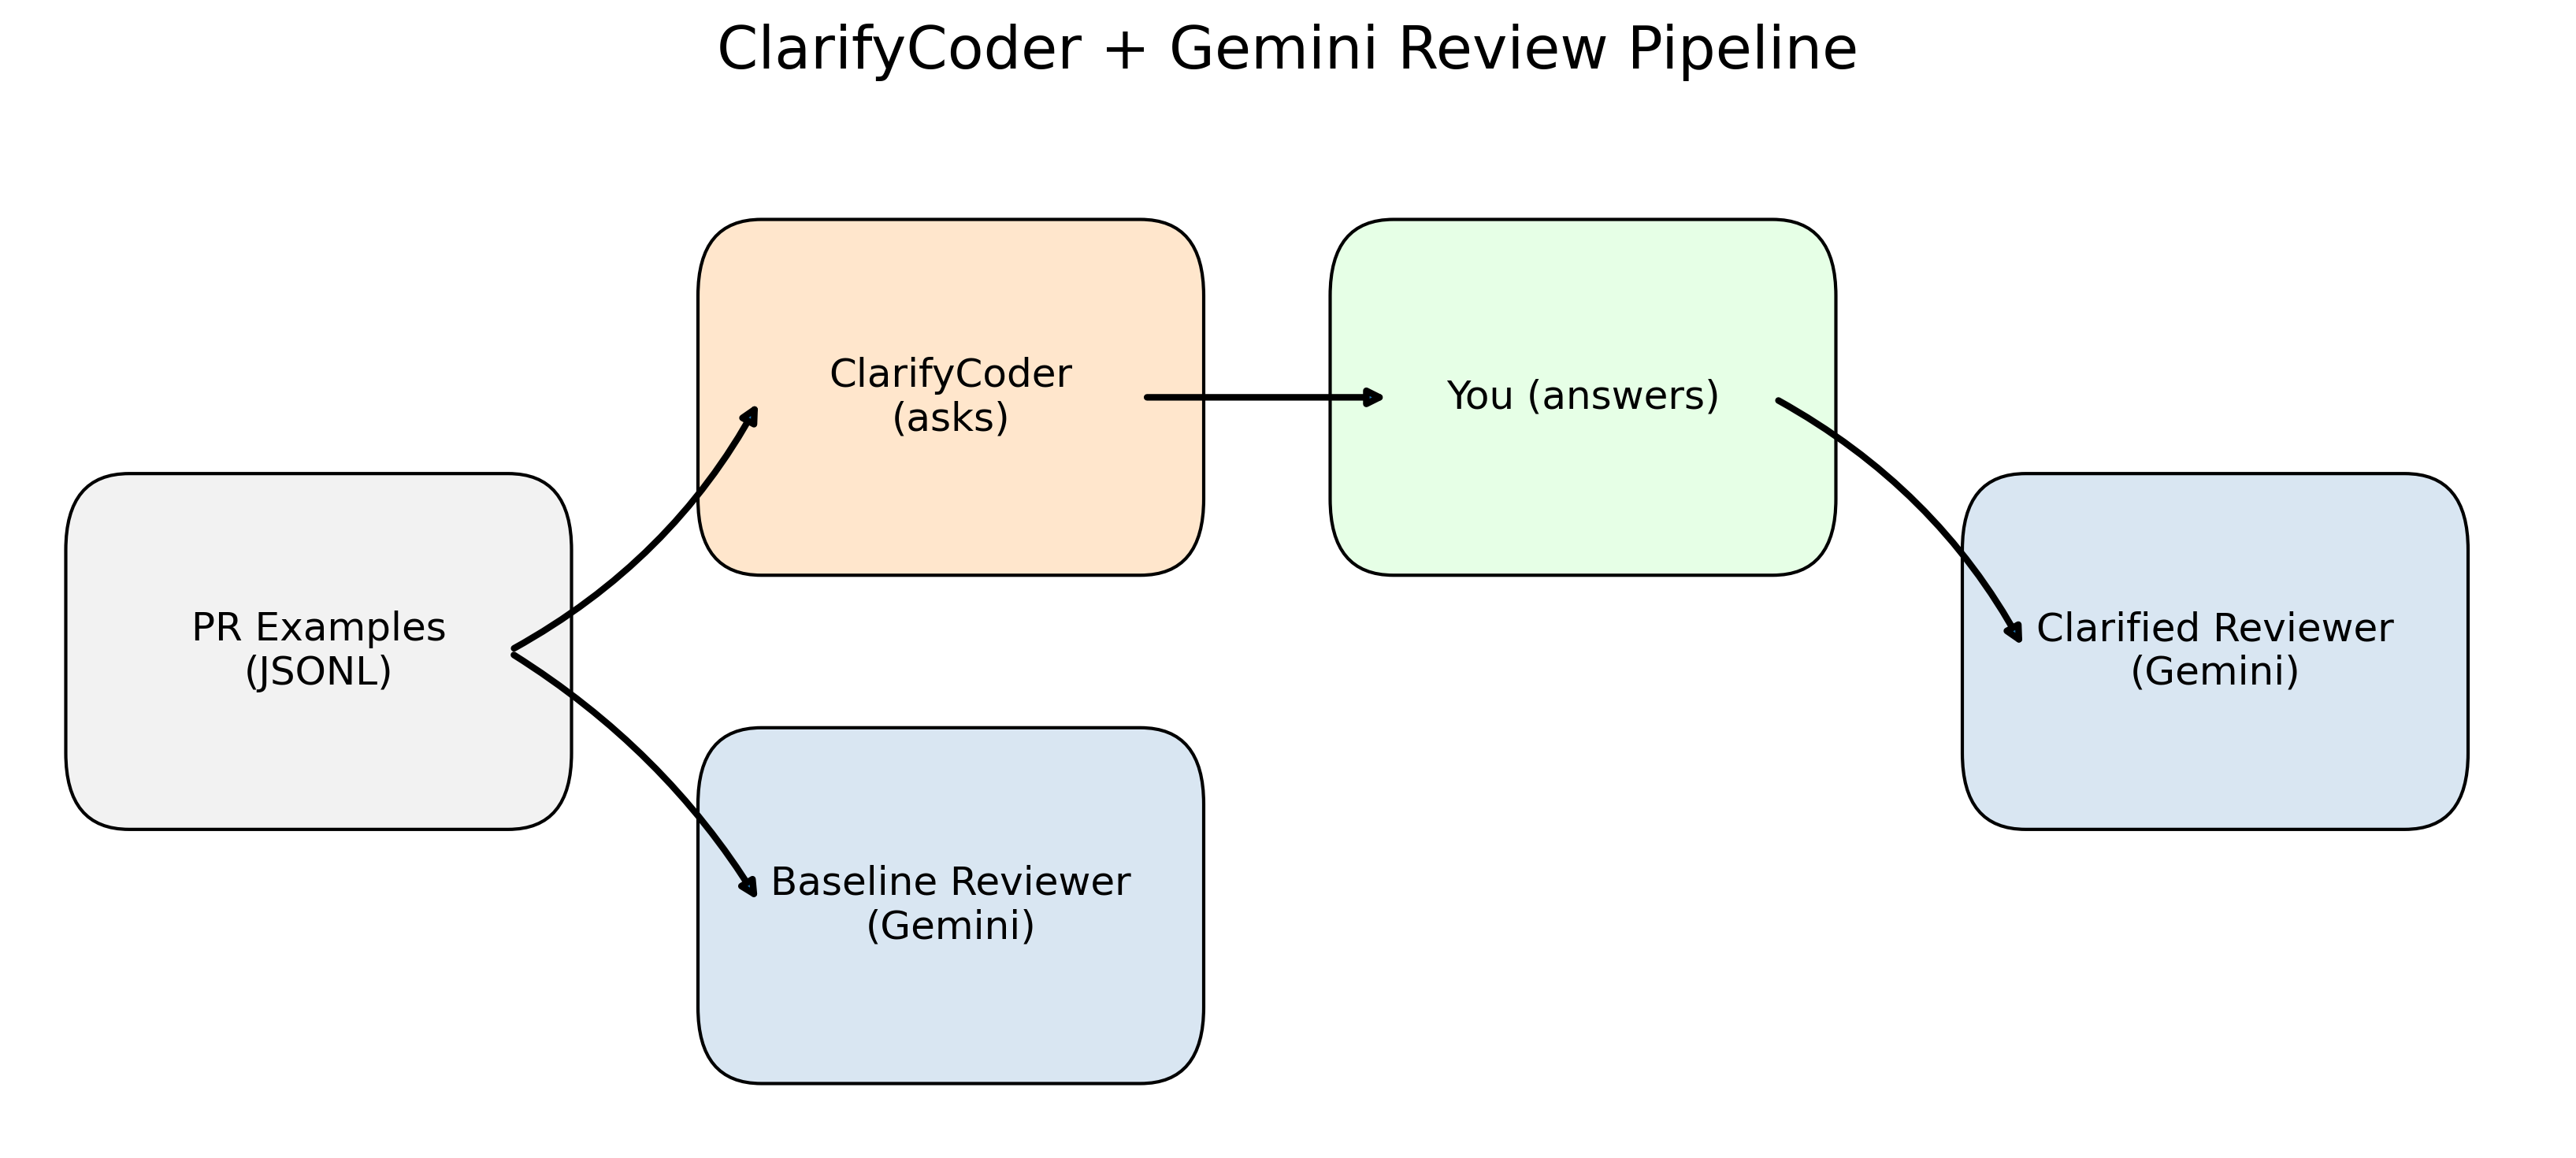
\includegraphics[width=\linewidth]{../results/plots/fig_architecture.png}
  \caption{Pipeline: PRs → ClarifyCoder (asks) → human answers → Clarified review.
  Baseline review runs in parallel; we compare outputs and score.}
  \label{fig:arch}
\end{figure}

\subsection{Artifacts}
The workflow produced several reproducible artifacts:
\begin{itemize}[leftmargin=*]
    \item Clarifying questions: \texttt{questions.tsv}
    \item Manual answers: \texttt{answers.tsv}
    \item Reviews: \texttt{baseline.jsonl}, \texttt{clarified.jsonl}
    \item Side-by-side comparison: \texttt{comparison.tsv}
    \item Scored evaluations: \texttt{eval\_scored.tsv}, \texttt{eval\_summary.tsv}
\end{itemize}
These files, along with the code scripts, ensure transparency and reproducibility.

\subsection{Metrics}
Each review was evaluated using five metrics:
\begin{itemize}[leftmargin=*]
    \item \textbf{Specificity (1--5):} How concrete and precise the comments are.
    \item \textbf{Actionability (1--5):} How directly usable the feedback is for making changes.
    \item \textbf{Assumptions identified (count):} Number of implicit assumptions surfaced explicitly.
    \item \textbf{Comment quality (1--5):} Overall usefulness of the review.
    \item \textbf{Suggestions (count):} Number of distinct, actionable suggestions provided.
\end{itemize}
This scoring scheme provided both quantitative and qualitative insight into the effect of clarification.


\section{Dataset}
We used 12 PRs spanning different modules. ClarifyCoder generated on average one clarifying question per PR, which were answered with an average length of 33 tokens.

\begin{table}[h]
\centering
\caption{Corpus statistics.}
\begin{tabular}{ll}
\toprule
PRs (n) & 12 \\
Avg. clarifying questions per PR & 1.0 \\
Avg. answer length (tokens) & 33 \\
\bottomrule
\end{tabular}
\end{table}

\section{Results}
\subsection{Quantitative Results}
We report averages across 12 PRs for five review metrics. Clarified
reviews outperform the baseline on every metric; detailed values and
per-metric deltas are shown below in figure 2 and figure 3.
\begin{figure}[t]
  \centering
  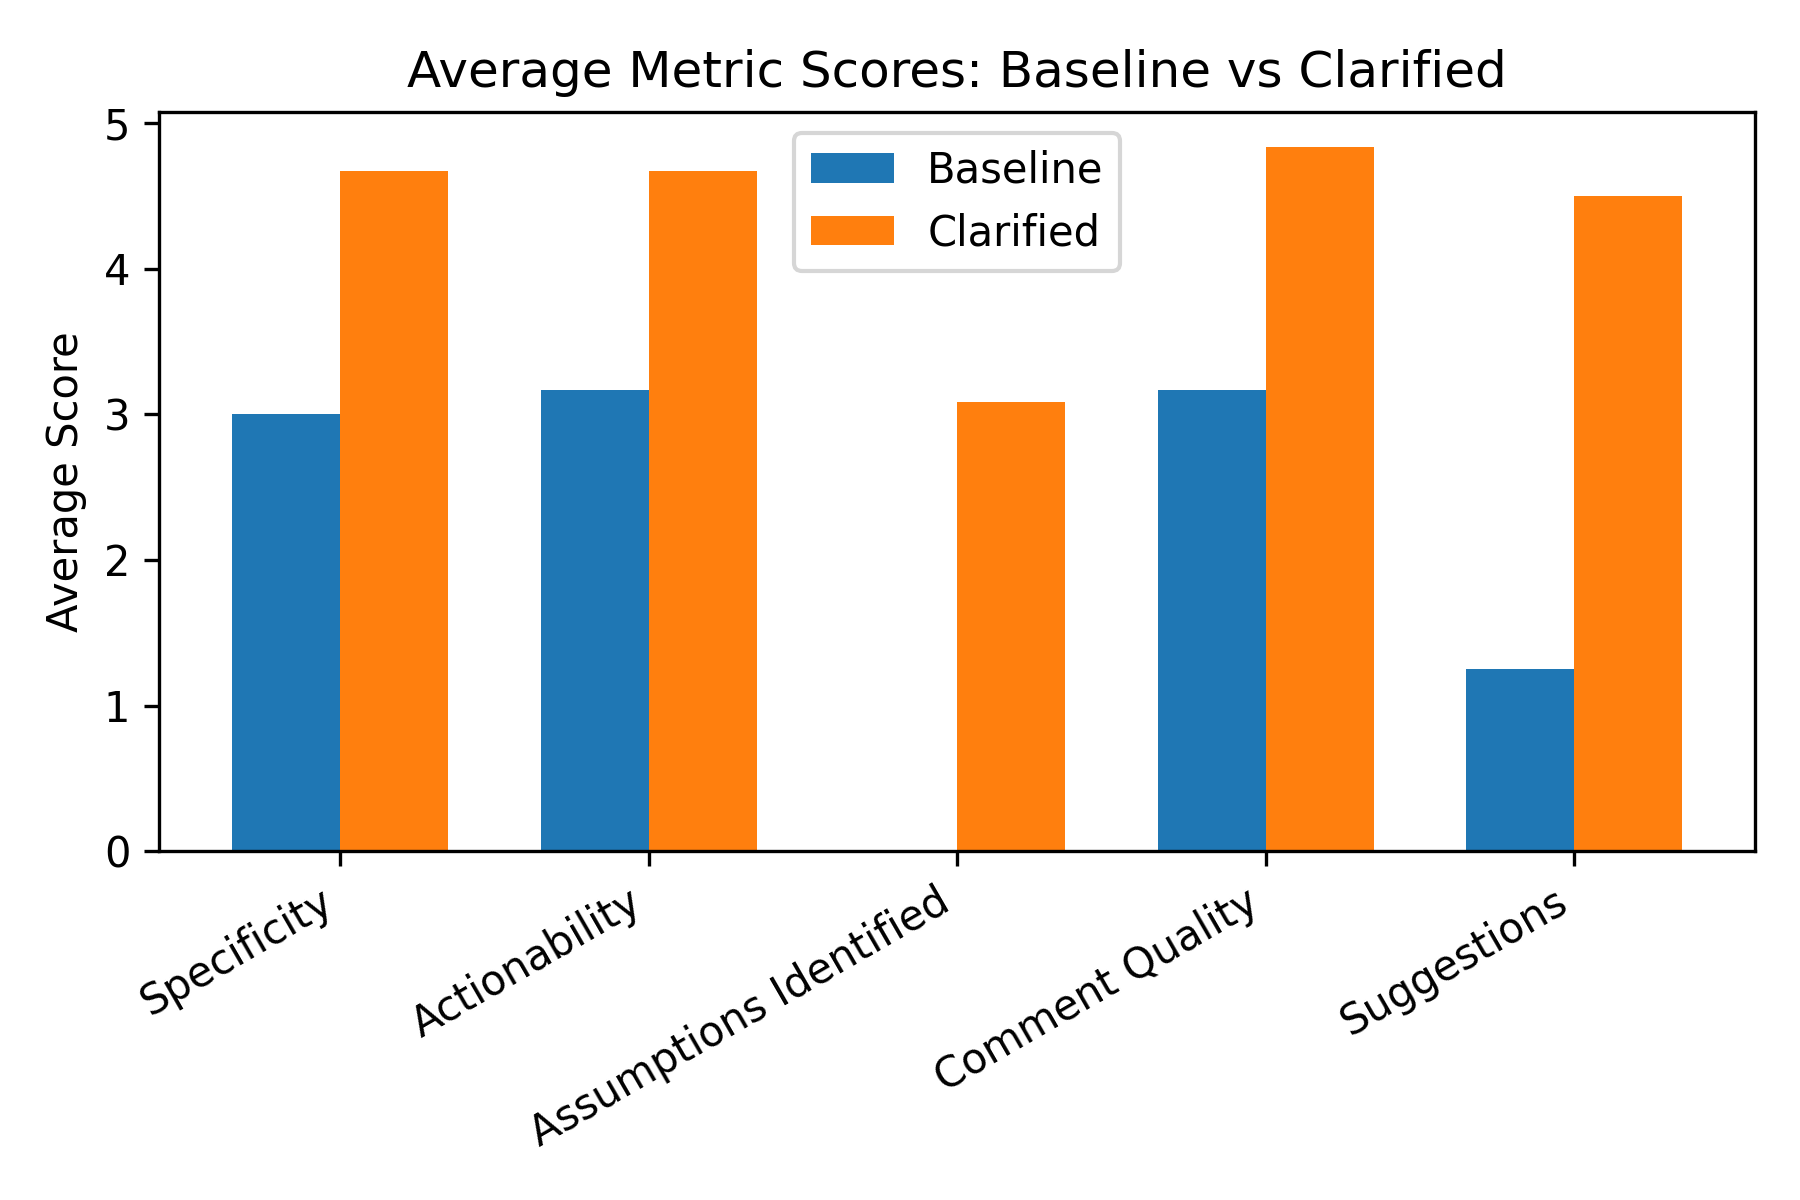
\includegraphics[width=\linewidth]{../results/plots/fig_metrics_bars.png}
  \caption{Average scores across 12 PRs}
  \label{fig:metrics}
\end{figure}

\begin{table}[h]
\centering
\caption{Mean scores (Clarified vs Baseline).}
\begin{tabular}{lrrr}
\toprule
Metric & Baseline & Clarified & $\Delta$ \\
\midrule
Specificity & 3.00 & 4.67 & +1.67 \\
Actionability & 3.17 & 4.67 & +1.50 \\
Assumptions Identified & 0.00 & 3.08 & +3.08 \\
Comment Quality & 3.17 & 4.83 & +1.67 \\
Suggestions & 1.25 & 4.50 & +3.25 \\
\bottomrule
\end{tabular}
\end{table}

\begin{figure}[t]
  \centering
  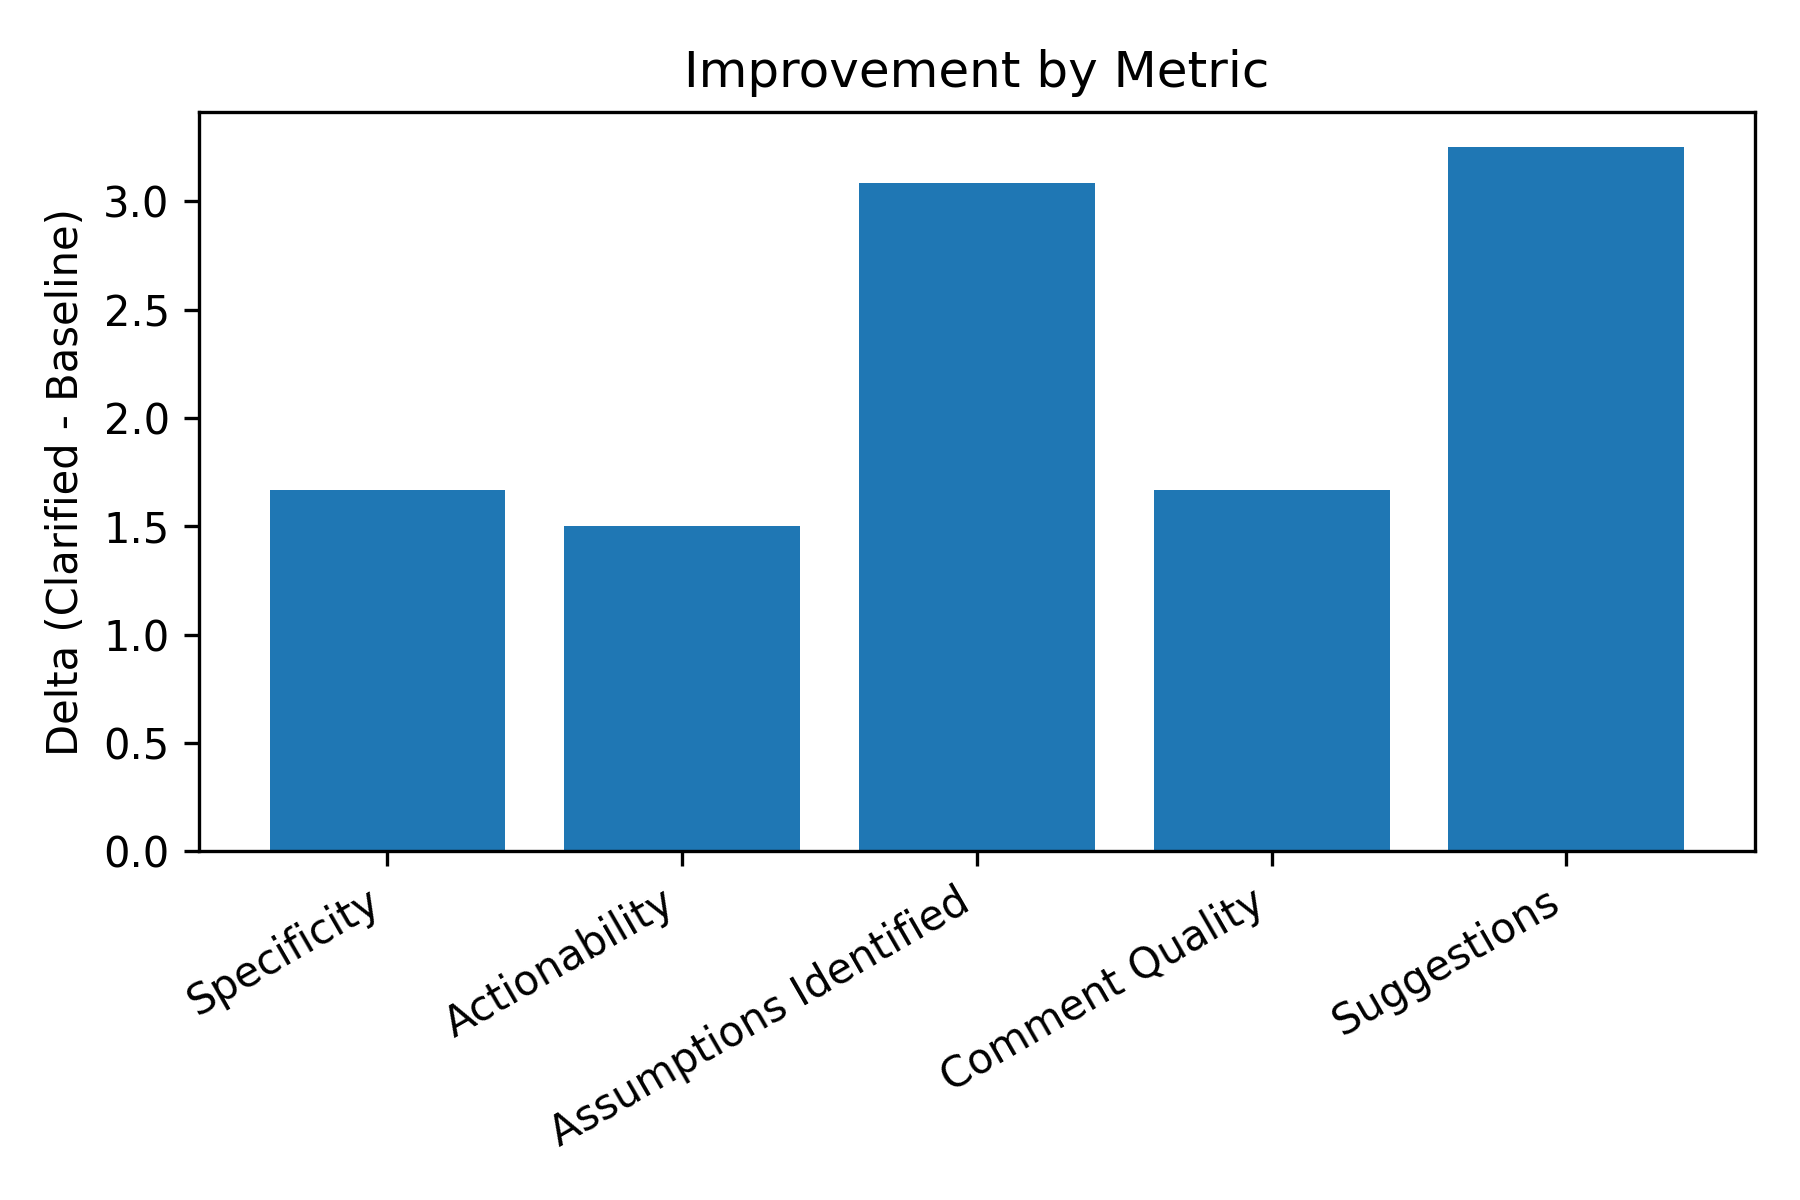
\includegraphics[width=\linewidth]{../results/plots/fig_delta_bars.png}
  \caption{Per-metric improvements after clarification (Clarified - Baseline).}
  \label{fig:deltas}
\end{figure}


\subsection{Qualitative Examples}
Two illustrative examples demonstrate the improvement:

\textbf{PR 0 -- Improve List Scoring Logic}\\
\emph{Baseline Review:} Asked vaguely for more detail on scoring algorithm, performance, and tests.\\
\emph{Clarified Review:} Explicitly demanded the scoring formula, handling of type stability, canonicalization rules, and comprehensive test coverage with examples.

\textbf{PR 1 -- Better User Status}\\
\emph{Baseline Review:} Requested clarification on how ``active'' is redefined and tests.\\
\emph{Clarified Review:} Demanded explicit decay function definition, threshold justification, performance evaluation, and detailed test cases.

These examples show how clarification transformed vague requests into detailed, actionable feedback.

\section{Discussion}
The evaluation results demonstrate consistent improvements when clarification was introduced. Across 12 PRs, clarified reviews achieved higher mean scores in every metric (Table~\ref{tab:means}). Specificity increased by +1.67, actionability by +1.50, and comment quality by +1.67. Most notably, clarified reviews explicitly identified assumptions (mean 3.08) compared to none in baseline reviews. Suggestions also increased substantially, from an average of 1.25 per PR to 4.5 (+3.25). These gains confirm the hypothesis that a clarification step improves the grounding and usefulness of AI-generated code reviews.

Qualitative analysis from the comparison file further illustrates these improvements. For example, in PR~0 (\emph{Improve list scoring logic}), the baseline review vaguely asked for “more detail” on scoring, whereas the clarified review explicitly demanded a scoring formula, type stability handling, and detailed test coverage. Similarly, in PR~1 (\emph{Better user status}), the baseline only asked how “active” was defined, while the clarified review insisted on a decay function definition, threshold justification, and performance evaluation. These examples show how clarification transformed generic requests into concrete, actionable feedback.

At the same time, not all improvements were uniform. In some cases, such as PR~3 (\emph{Improve error reporting}), both baseline and clarified reviews remained somewhat vague, suggesting that clarification quality depends on the relevance of generated questions.

Overall, the evidence indicates that clarification strengthens reviews by reducing hallucination, exposing assumptions, and producing richer feedback. However, further refinement of the clarifier model and exploration of automated answering will be needed for real-world deployment.

\section{Limitations and Future Work}
This study has several limitations. First, clarifying questions were answered manually, which ensured quality but may not scale; automating this step could introduce noise or inconsistency. Second, the evaluation was limited to twelve PRs, so larger and more diverse datasets are needed to confirm generalizability. Finally, improvements depend heavily on the relevance of ClarifyCoder’s questions, which varied across examples.  
Future work should explore (1) automating the answering step, (2) fine-tuning reviewers to incorporate clarifications directly, and (3) testing at scale in real-world developer environments.

\section{Conclusion}
This work tested a simple but effective intervention: inserting a clarification phase into AI code review. By combining ClarifyCoder (to generate questions) with Gemini (to generate reviews), and by manually answering clarifying questions, we were able to improve review specificity, actionability, assumption identification, comment quality, and suggestion count. Both quantitative metrics and qualitative examples confirm the effectiveness of this approach.

The main contribution of this study is to show that clarification, previously validated in program synthesis, also transfers effectively to a developer-facing environment: pull request review. The results suggest that lightweight clarification mechanisms can make AI reviewers substantially more useful in practice.

In summary, adding a clarification phase leads to reviews that are more grounded, informative, and aligned with developer needs. This provides a promising direction for building next-generation AI-assisted code review systems.

\bibliographystyle{IEEEtran}
\bibliography{refs}

\end{document}
